\documentclass[11.5pt, paper=a4]{article}

\usepackage[utf8]{inputenc}
\usepackage[english]{babel}
\usepackage[T1]{fontenc}

\usepackage{amsmath, amssymb, amscd, amsthm, amsfonts, mathtools}
\usepackage[left=2cm, right=2cm, top=1.5cm]{geometry}

\usepackage{graphicx}
\usepackage{hyperref}
\usepackage{physics}
\usepackage{tikz}
\usepackage{url}
\usepackage[square,numbers]{natbib} \usepackage{tabularx}
\usetikzlibrary{quantikz}

\usepackage{braket}
\usepackage{thmtools}
\usepackage{float}

%%% Theorem Style
\theoremstyle{definition}
\newtheorem{theorem}{Theorem}[section]
\newtheorem{definition}[theorem]{Definition}
\newtheorem{lemma}[theorem]{Lemma}
\newtheorem{conjecture}[theorem]{Conjecture}
\newtheorem{corollary}[theorem]{Corollary}

\numberwithin{theorem}{section}

%% Autoref prefixes
\renewcommand{\sectionautorefname}{Section}
\renewcommand{\subsectionautorefname}{Section}
\renewcommand{\subsubsectionautorefname}{Section}
\renewcommand{\figureautorefname}{Figure}
\def\theoremautorefname{Theorem}
\def\lemmaautorefname{Lemma}
\def\definitionautorefname{Definition}
\def\conjectureautorefname{Conjecture}
\def\algorithmautorefname{Algorithm}

%% Writing algorithms

\usepackage{algorithm} % captioning 
\usepackage{algpseudocode}

% \def\NoNumber#1{{\def\alglinenumber##1{}\State #1}\addtocounter{ALG@line}{-1}}



\title{Quantum Algorithms, Spring 2022: Lecture 6 Scribe}

\author{Rutvij Menavlikar, Abhyudit Mohla}

\date{January 25, 2022}

\begin{document}

\maketitle

\section{Recap}

\subsection{Universality of Quantum Circuits}

\begin{itemize}
    \item Single qubit and $CNOT$ gates together can be used to implement an arbitrary two-level unitary operation on the state space of $n$ qubits.\cite{nielsen_chuang}
    \item The set $\{CNOT,H,R_{\frac{\pi}{4}}\}$ is universal for quantum computing, i.e. any other quantum circuit can be well approximated using quantum circuits of only these gates.\\And \emph{Solovay-Kitaev thoerem} states that any $t$-gate quantum circuit can be $\epsilon$ approximated using\\ $\mathcal{O}\left(t.\text{polylog}\left(\frac{1}{\epsilon}\right)\right)$ gates from $\{CNOT,H,R_{\frac{\pi}{4}}\}$.
\end{itemize}

\subsection{Quantum Parallelism}

To estimate a function $f$ s.t.
\begin{equation*}
f:\{0,1\}^n\rightarrow\{0,1\}
\end{equation*}
we use a quantum gate $U_f$ in the following way.
\begin{center}
\begin{quantikz}
\lstick{$\ket x$} & \gate[wires=2][2cm]{U_f} & \qw & \rstick{$\ket x$} \\
\lstick{$\ket y$} & & \qw & \rstick{$\ket{y\oplus f(x)}$}
\end{quantikz}
\end{center}
\begin{equation}
\begin{split}
\text{So, }&\text{if }f(x)=0\text{, }\ket x\ket y\xrightarrow{U_f}\ket x\ket y\\
&\text{if }f(x)=1\text{, }\ket x\ket y\xrightarrow{U_f}\ket x\ket{\bar y}
\end{split}
\end{equation}

Now, we can parallelise this circuit, even for $n$ qubits by adding Hadamard's gates on input qubits before applying the $U_f$ gate in the following way.
\begin{center}
\begin{quantikz}
\lstick[wires=4]{$N$} & \lstick{$\ket 0$} & \gate{H} & \gate[wires=5][5cm]{U_f} & \qw \\
 & \lstick{.} & \gate{H} & & \qw \\
 & \lstick{.} & \gate{H} & & \qw \\
 & \lstick{$\ket 0$} & \gate{H} & & \qw \\
\lstick{$\ket 0$} & & \qw & & \qw
\end{quantikz}
\end{center}

Thus, by applying $U_f$ only once, we are able to obtain a quantum state that contains all possible $2^n$ values of $f(x)$ in superposition.
\begin{equation}
\ket{0}^{\otimes n}\ket 0\xrightarrow{H^{\otimes n}\otimes I}\frac{1}{\sqrt{2^n}}\sum_{x\in \{0,1\}^n}\ket x\ket 0\xrightarrow{U_f}\frac{1}{\sqrt{2^n}}\sum_{x\in \{0,1\}^n}\ket x\ket{f(x)}
\end{equation}

Note that,
\begin{itemize}
    \item Quantum parallelism is not enough to demonstrate the power of Quantum Computing
    \item Quantum parallelism needs to be combined with interference, entanglement to do something better than classical computing.
\end{itemize}

\subsection{Deutsch Algorithm}

\subsubsection{Problem}

We are given a binary function $f:\{0,1\}\rightarrow\{0,1\}$ such that either $f(0)=f(1)$ or $f(0)\neq f(1)$. We have determine which using minimum number of queries.

\subsubsection{Classical Approach}
We query for value of $f(0)$ and $f(1)$ to determine which kind of function is $f$.\\
Hence, classical approach requires \emph{2} queries.

\subsubsection{Quantum Algorithm}
We set up the following circuit
\begin{center}
\begin{quantikz}
\lstick{$\ket 0$} & \gate{H} & \gate{U_f^{\pm}} & \gate{H} & \meter{0/1} \\
\end{quantikz}
\end{center}
The calculations are as follows
\begin{multline}
\ket 0\xrightarrow{H}\frac{1}{\sqrt 2}\left(\ket0+\ket1\right)\xrightarrow{U_f^{\pm}}\frac{1}{\sqrt 2}\left((-1)^{f(0)}\ket0+(-1)^{f(1)}\ket1\right)\xrightarrow{H}\\\frac{1}{2}\left(\left((-1)^{f(0)}+(-1)^{f(1)}\right)\ket0+\left((-1)^{f(0)}-(-1)^{f(1)}\right)\ket1\right)
\end{multline}
Thus, when $f(0)=f(1)$ the measured state is $\ket 0$, and when $f(0)\neq f(1)$ the measured state is $\ket 1$.\\
And hence, with quantum parallelism we can solve the problem with only 1 query to $U_f$.



\section{Mach-Zehnder Interferometer}
In physics, the Mach–Zehnder interferometer is a device used to determine the relative phase shift variations between two collimated beams derived by splitting light from a single source.\cite{Wikipedia} Essentially, Mach-Zehnder Interferometer physically captures Deutsch's problem.
\begin{figure}[H]
\centering
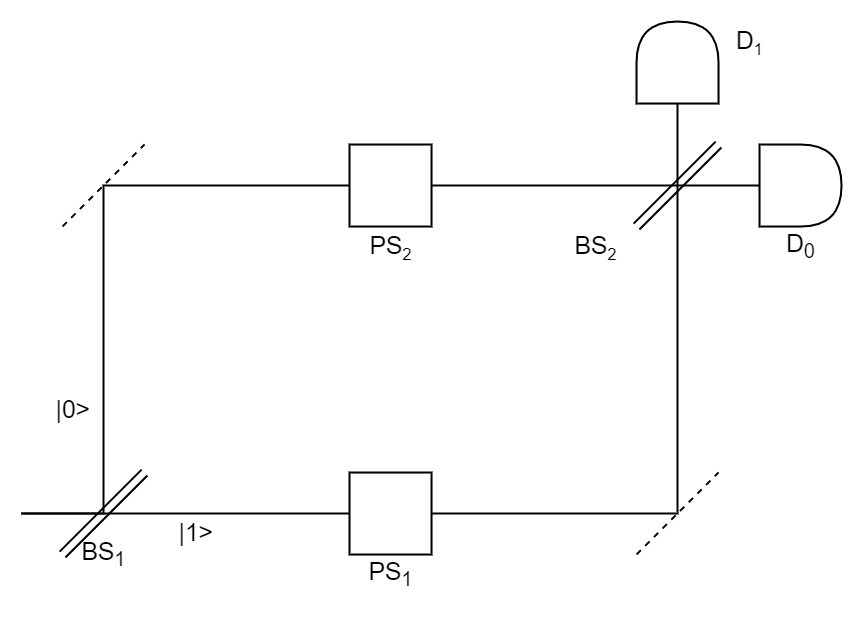
\includegraphics[width=0.9\textwidth]{images/Mach-Zehnder Interferometer.png}
\caption{Mach-Zehnder Interferometer set up}
\label{fig:1}
\end{figure}
The set up includes the following components
\begin{itemize}
\item $BS_1$ and $BS_2$ are beam splitters. They split a photon into a superposition of \emph{lower path} and \emph{upper path}.
\item $PS_1$ and $PS_2$ are phase shifters. $PS_1$ shifts the phase of the beam incident on it by $\phi_1$ and $PS_2$ shifts it by $\phi_0$.
\item $D_0$ and $D_1$ are detectors. $D_0$ detects a photon in \emph{lower path} and $D_1$ detects a photon in \emph{upper path}.
\end{itemize}

These components are arranged as shown in fig \ref{fig:1}.

Here we assume that \emph{lower path} is represented by $\ket0$ and \emph{upper path} is represented by $\ket1$. Thus, $\ket0$ undergoes phase shift of $\phi_0$ and $\ket1$ undergoes phase shift of $\phi_1$. This can be represented as
\begin{equation*}
\ket0\xrightarrow{PS_2}e^{i\phi_0}\ket0,\ket1\xrightarrow{PS_1}e^{i\phi_1}\ket1
\end{equation*}
Also, it is given that $\left|\phi_0-\phi_1\right|=0$ or $\pi$ and we have to determine which.

Thus, the calculations are as follows:
\begin{equation}
\ket0\xrightarrow{BS_1}\frac{1}{\sqrt2}\left(\ket0+\ket1\right)\xrightarrow{PS}\frac{1}{\sqrt2}\left(e^{i\phi_0}\ket0+e^{i\phi_1}\ket1\right)\xrightarrow{BS_2}\frac{1}{2}\left(\left(e^{i\phi_0}+e^{i\phi_1}\right)\ket0+\left(e^{i\phi_0}-e^{i\phi_1}\right)\ket1\right)
\end{equation}

But we can see that
\begin{equation}
\frac{1}{2}\left(\left(e^{i\phi_0}+e^{i\phi_1}\right)\ket0+\left(e^{i\phi_0}-e^{i\phi_1}\right)\ket1\right)=\frac{e^{i\phi_0}}{2}\left(\left(1+e^{i\left(\phi_1-\phi_0\right)}\right)\ket0+\left(1-1+e^{i\left(\phi_1-\phi_0\right)}\right)\ket1\right)
\end{equation}

Thus,
\begin{itemize}
\item When $\left|\phi_0-\phi_1\right|=0$, $\ket0$ is observed, i.e. $D_0$ detects a photon.
\item When $\left|\phi_0-\phi_1\right|=\pi$, $\ket1$ is observed, i.e. $D_1$ detects a photon.
\end{itemize}

\emph{Note that:} This is a quantum phenomena. Classically, each of the detector would detect a photon 50\% of the times.



\section{Deutsch-Jozsa Algorithm}
This algorithm is a generalisation of Deutsch problem on $n$ qubits.

\subsection{Problem}
We are given a black box $U_f$ for some Boolean function $f:\{0,1\}^n\rightarrow\{0,1\}$ where it is given that $f$ is either \emph{constant} or \emph{balanced}, i.e
\begin{align*}
\text{Either, }&f(x)=\emph{ constant: }\forall x\in\{0,1\}^n,f(x)=e\text{ s.t. }e\in\{0,1\}\\
&f(x)=\emph{ balanced: }
\begin{cases}
0,&\text{for }2^{n-1}\text{ values of }x\\
1,&\text{for rest of the }2^{n-1}\text{ values of }x
\end{cases}
\end{align*}
We have to determine which using minimum number of queries.

\subsection{Classical Approach}
Serially, or randomly we input values of $x\in\{0,1\}^n$ and check their outputs.
\begin{itemize}
    \item If $f$ is \emph{balanced}:\\If we observe 0 and 1 in output, then $f$ is \emph{balanced}. And by Pigeonhole principle, we would require at-most $2^{n-1}+1$ queries to reach this conclusion.
    \item If $f$ is \emph{constant}:\\If we observe the same output after $2^{n-1}+1$ queries, we can conclude that $f$ is \emph{constant}.
\end{itemize}
Hence, number of queries required are $2^{n-1}+1$.

\subsection{Quantum Algorithm}
We set up the following circuit
\begin{center}
\begin{quantikz}
\lstick[wires=4]{$n$} & \lstick{$\ket 0$} & \gate[wires=4][2cm]{H^{\otimes n}} & \gate[wires=4][4cm]{U_f^{\pm}} & \gate[wires=4][2cm]{H^{\otimes n}} & \meter{0/1} \\
 & \lstick{.} & & & & \meter{0/1} \\
 & \lstick{.} & & & & \meter{0/1} \\
 & \lstick{$\ket 0$} & & & & \meter{0/1}
\end{quantikz}
\end{center}
This leads to the following changes,
\begin{multline}
\ket 0^{\otimes n}\xrightarrow{H^{\otimes n}}\frac{1}{\sqrt{2^n}}\sum_{x\in\{0,1\}^n}\ket x\xrightarrow{U_f^{\pm}}\frac{1}{\sqrt{2^n}}\sum_{x\in\{0,1\}^n}(-1)^{f(x)}\ket x\xrightarrow{H^{\otimes n}}\frac{1}{2^n}\sum_{x\in\{0,1\}^n}\sum_{z\in\{0,1\}^n}(-1)^{f(x)+x.z}\ket z
\end{multline}
Let $\ket{\psi_f}=\frac{1}{2^n}\sum_{x\in\{0,1\}^n}\sum_{z\in\{0,1\}^n}(-1)^{f(x)+x.z}\ket z$\\
Then, we look at the amplitude of $\ket 0^{\otimes n}$ in $\ket{\psi_f}$,
\begin{align}
\braket{00..0|\psi_f}&=\frac{1}{2^n}\sum_{x\in\{0,1\}^n}\sum_{z\in\{0,1\}^n}(-1)^{f(x)+x.z}\braket{00..0|z}\\
&=\frac{1}{2^n}\sum_{x\in\{0,1\}^n}(-1)^{f(x)}&&\braket{00..0|z}=
\begin{cases}
1,&z=\ket0^{\otimes n}\\
0,&\text{otherwise}
\end{cases},x.0=0
\end{align}
Thus,
\begin{itemize}
    \item If $f$ is \emph{balanced}:\\$\braket{00..0|\psi_f}=0$
    \item If $f$ is \emph{constant}:\\$\braket{00..0|\psi_f}=1$ or $\braket{00..0|\psi_f}=-1$
\end{itemize}
Thus, if the result of measurement is the state $\ket0^{\otimes n}$, then $f$ is \emph{constant}, and for any other result of measurement $f$ is \emph{balanced}.\\
Hence, only 1 query is required to classify the function. And hence, there is an exponential optimization in query complexity.

\subsection{Randomized Deutsch-Jozsa Algorithm}
Now, we require our algorithm to classify $f$ with a probability $\geq1-\epsilon$ ($\epsilon>0$)

\subsubsection{Classical Approach}
We choose $d$ values of $x\in\{0,1\}^n$ to query.
\begin{align*}
\text{Let values of }x\text{: }S&=\{x_1,x_2,..,x_d\}&&x_i\in\{0,1\}^n
\end{align*}
Thus, by making the $d$ queries, we get $f(S)=\{f(x_1),f(x_2),..,f(x_d)\}$
Then the following scenarios are possible,
\begin{itemize}
    \item \emph{Case 1}: $\forall x_i\in S,f(x_i)=0$ or $\forall x_i\in S,f(x_i)=1$\\In this case, if $d<2^{n-1}+1$, then we still cannot be sure is $f$ is \emph{balanced} or \emph{constant}. And hence, there is an uncertainty in classification. But the probability of observing this case is $\frac{1}{2^d}+\frac{1}{2^d}=\frac{1}{2^{d-1}}$
    \item \emph{Case 2}: $\exists x_i,x_j\in S,$ s.t. $f(x_i)\neq f(x_j)$\\In this case, we can definitely conclude that $f$ is \emph{balanced}.
\end{itemize}
Thus, we can choose $d$ in a way that we reduce the probability of observing the case where we are not certain about the outcome. That is,
\begin{equation}
\frac{1}{2^{d-1}}<1-(1-\epsilon)\Rightarrow d>\log_2\left(\frac{2}{\epsilon}\right)
\end{equation}
Hence, the query complexity for the classical approach to the randomised Deutsch-Jozsa Problem is $\mathcal{O}\log\left(\frac{1}{\epsilon}\right)$



\section{Bernstein-Vazirani Algorithm}
A related problem was given by Ethan Bernstein and Umesh Vazirani.

\subsection{Problem}
We are given a black box $U_f$ for some Boolean function $f:\{0,1\}^n\rightarrow\{0,1\}$ where it is given that $\forall x\in \{0,1\}^nf(x)=s.x(\mod2)$ for some unknown string $s\in \{0,1\}^n$. i.e.,
\begin{equation*}
\forall x\in \{0,1\}^nf(x)=s_1x_1\oplus s_2x_2\oplus...\oplus s_nx_n
\end{equation*}
We have to determine $s$ using minimum number of queries.

\subsection{Classical Approach}
We pass a set of inputs $I=\{x_1,x_2,..,x_n\}$ such that
\begin{equation*}
\forall x_i\in I,x_i(j)=
\begin{cases}
1,&j=i\\
0,&\text{otherwise}
\end{cases}
\end{equation*}
Thus, the output of each input $x_i$ looks like
\begin{align}
f(x_i)&=s_1x_i(1)\oplus s_2x_i(2)\oplus..\oplus s_nx_i(n)\\
&=0\oplus0\oplus..\oplus0\oplus s_i\oplus0\oplus..\oplus0\\
&=s_i
\end{align}
Hence, $n$ queries are required to determine $s$.

\subsection{Quantum Algorithm}
We set up the circuit in the same way as we did for Deutsch-Jozsa Algorithm.
\begin{center}
\begin{quantikz}
\lstick[wires=4]{$n$} & \lstick{$\ket 0$} & \gate[wires=4][2cm]{H^{\otimes n}} & \gate[wires=4][4cm]{U_f^{\pm}} & \gate[wires=4][2cm]{H^{\otimes n}} & \meter{0/1} \\
 & \lstick{.} & & & & \meter{0/1} \\
 & \lstick{.} & & & & \meter{0/1} \\
 & \lstick{$\ket 0$} & & & & \meter{0/1}
\end{quantikz}
\end{center}
The calculations are as follows,
\begin{equation}
\ket 0^{\otimes n}\xrightarrow{H^{\otimes n}}\frac{1}{\sqrt{2^n}}\sum_{x\in\{0,1\}^n}\ket x\xrightarrow{U_f^{\pm}}\frac{1}{\sqrt{2^n}}\sum_{x\in\{0,1\}^n}(-1)^{f(x)}\ket x
\end{equation}
and
\begin{align}
\frac{1}{\sqrt{2^n}}\sum_{x\in\{0,1\}^n}(-1)^{f(x)}\ket x&=\frac{1}{\sqrt{2^n}}\sum_{x\in\{0,1\}^n}(-1)^{x.s(\mod2)}\ket x\\
&=\frac{1}{\sqrt{2^n}}\sum_{x\in\{0,1\}^n}(-1)^{x.s}\ket x
\end{align}
But note that $\ket s\xrightarrow{H^{\otimes n}}\frac{1}{\sqrt{2^n}}\sum_{x\in\{0,1\}^n}(-1)^{x.s}\ket x$ and $H^{\otimes n}\times H^{\otimes n}=\mathbb{I}_n\Rightarrow \left(H^{\otimes n}\right)^{-1}=H^{\otimes n}$\\
Thus,
\begin{equation}
\frac{1}{\sqrt{2^n}}\sum_{x\in\{0,1\}^n}(-1)^{f(x)}\ket x\xrightarrow{H^{\otimes n}}\ket s
\end{equation}
Hence, the measured output is the string $s$.\\
And hence, we are able to determine $s$ in 1 query, which gives us a linear speed up in query complexity.

\bibliographystyle{plainnat}
\bibliography{references}

\end{document}

